%!TEX root = ../master.tex
\chapter{Designing the Learning Activity}
\label{chap:designing_learning_acitivty}
%!TEX root = ../../master.tex
\begin{theorem}
Designing a learning activity is necessary to investigate the effects of KubeCloud. Learning theories must be applied within the constraints of the course format.
\end{theorem}

\noindent
Chapter \ref{chap_fundamentals_learning} covered some of the fundamentals of learning theory. In this chapter, we will apply these theories and concepts to design a learning activity focused on the use of a tangible cloud computing cluster. We propose a design of a learning activity using a tangible cloud computing cluster as a learning object. The focus of the learning activity is to motivate and engage students in practical problem solving in cloud computing. The following chapters will give a detailed explanation of the concepts and theories the designed learning activity is based on. \\

\noindent 
The designed learning activity has been taught in a course, Object-Oriented Network Communication\footnote{\url{http://kursuskatalog.au.dk/en/course/63876}} at Aarhus University School of Engineering,  to verify the learning outcome of the learning activity and the impact of the tangible cloud computing cluster. These results will be presented in Chapter~\ref{chapter_experiment2_resilience}, \ref{chapter_experiment1_learning_experience}.
%!TEX root = ../../master.tex
\section{The Need for a Learning Object}
Activity-based theories describe the use of learning objects and the importance such an object can have in a learning experience. We see a need for designing a learning object that can help students understand the context from which many abstractions in cloud computing have been made, and propose \textit{KubeCloud - A Small-Scale Tangible Cloud Computing Environment}.\\

\noindent
Abstractions are one of the key concepts in cloud computing, and these abstractions have made it easy for developers to provision and deploy applications in the cloud. Failing to understand the premise of these abstractions can have great consequences. The paradigm shift from monolithic applications (using intra-process method calls) to multiple small services (using inter-process communication over a network) introduces a lot of complexity that has to be dealt with. The fallacies of distributed computing have to be addressed and made visible for students. KubeCloud will help students learn about the fallacies of distributed programming and provide a platform for experimentation and exploration in a controlled environment. An active process, in which the learner uses sensory input and constructs meaning out of it, is important (Chapter~\ref{chap_fundamentals_learning}). This view is also pointed out by Satterthwait, \textit{"Some of the most productive, and common, science activities are those that involve the manipulation of objects. This factor plays a significant role in motivating and focusing our students on the learning of Science through the use of objects in an activity in which they can be engaged"} \cite[p. 8]{satterthwait2010hands}. The need for hands-on experience was found in a survey conducted at Jordan University of Science and Technology during an investigation into the challenges of teaching Cloud Computing. 93\% of the students answered that there was a lack of hands-on experience \cite[p. 2]{jararweh2013teachcloud}. \\

\noindent
Chapter~\ref{chap:tangible_cluster} covers the details of the design of the KubeCloud. The course presented in this master's thesis will be designed around an active, student-based approach and the use of the tangible cloud computing cluster as an object for learning.


\section{Designing the Overall Learning Activity}

The course format is constrained, by an external requirement from the university, to have a duration of seven weeks. These seven weeks are derived into seven modules, each consisting of two half days (4x45min) with respectively lectures and project work. The designed course will be tested inside the scope of an already existing course; Object-Oriented Network Communication\footnote{\url{http://kursuskatalog.au.dk/da/course/63876}} taught by Christian Fischer Pedersen. Object-Oriented Network Communication restricts the design of the course since Domain Name Service (DNS) is presented in module 6 by Pedersen. DNS is, though, related to the rest of the course and plays an important role in the understanding of how the cluster management system, Kubernetes, performs service discovery. \\

\noindent 
As described in Chapter~\ref{chap_fundamentals_learning}, a learning activity involves three elements: learning outcomes, means, and assessment. The following section will first provide a high-level overview of the design of the course in its entirety, and afterward describe the design of the individual module, using these three elements as the primary structure.

\subsection*{Learning Outcomes}
Learning outcomes refer to the outcomes that the students should be able to achieve from the designed course. The topics of the course have been chosen to give the students an introduction to cloud computing, the movement towards a service-oriented architecture, and containerization of applications. The topics will be discussed later in this master's thesis. We will first describe the qualifications of the course designed using Bloom's taxonomy to assess the students' performance in the exam. Lastly, a more detailed description of the course content is supplied.

\subsubsection*{Description of Qualifications}
The participants will after the course have insight in the possibilities with state-of-the-art microservice architecture and the elements involved in deploying containerized services in a cloud computing platform. The course will focus on designing a microservice architecture based on the Spring Boot and Spring Cloud frameworks, containerizing the services with Docker and deploying the containerized architecture into a Container as a Service platform, Kubernetes. Emphasis will be on designing distributed systems in regards to resilience and error handling. \\

\noindent 
The participants must at the end of the course be able to: 
\begin{itemize}
  \item Judge and select appropriate strategies for handling perturbations in a distributed architecture
  \item Design and construct a distributed microservice architecture, containerize and deploy the system in a cloud computing platform
  \item Validate the distributed microservice architecture in relation to resilience
  \item Explore and compare different antipatterns in faults for distributed systems
  \item Reflect upon the state-of-the-art microservice architecture compared to a monolithic architecture
\end{itemize}

\subsubsection*{Contents}
The designed course presents an overview of fundamental principles of distributed systems and cluster computing with a particular focus on resilience in a microservice architecture. Containerizing services will be presented and discussed throughout the course with Docker as the enabling technology. Different deployment models will be presented and a Container as a Service platform will be used as the infrastructure for deploying containers. The course will give practical hands-on experience with running a microservice architecture in a Raspberry Pi Kubernetes cluster, KubeCloud. Resilience will be presented and discussed. Practical experience will be achieved using KubeCloud by pulling network cables and attacking the cluster. The DNS and service discovery part of the course will give an introduction to the fundamentals of DNS and explain how service discovery is an important concept when abstracting the underlying hardware with a cluster management system such as Kubernetes. The underlying theme of the course is a real-life problem that the students must solve using the presented concepts and theory.

\subsection*{Means}
Means refer to the actions instructors can take to provide the best possible learning experience for the students to achieve the learning outcomes. 

\subsubsection*{Determining Students' Learning Style}
The course is designed to foster the highest possible learning outcome for the students. This raises the need for insights into how the participating students describe their learning preferences. To gain this insight, the students are asked to hand in a questionnaire before the start of the course. The questionnaire is created by Felder\footnote{\url{http://www.engr.ncsu.edu/learningstyles/ilsweb.html}}, and the goal is to determine the students' learning style according to the theory described in Chapter~\ref{chap_fundamentals_learning}. The questionnaire consists of 44 questions. Each question has two possible answers and an answer to each question is required. Felder and Silverman describe engineering students to be sensory, visual, active and sequential learners. The result of the questionnaires filled out by the participating students shows that three out of four learning styles match the expected style. However, the students participating in the course lean towards a global learning style preferences instead. This preference must be addressed in the course design. Chapter~\ref{chapter_experiment1_learning_experience} gives a more detailed description of this experiment.


\subsubsection*{Teaching Style}
Knowing about the students' preference of learning styles, we can design the course to optimize their learning. The experiment shows that the students have a preference for the sensory learning style, which includes facts, data, and experimentation. This suggests that the use of a learning object for experimentation is the right approach. Using multiple sources of learning is a good way to cover the learning style preferences. For instance, this is achieved through a combination of presenting the topics in the form of facts and data, and then having the students experiment in workshops and project work. These methods point in the direction of a student-centered approach, which will include the students in a much higher degree. This approach is also supported by the students preferring an active learning style which involves using the information they obtain actively. A problem-based learning approach is chosen to apply the context of the real world. We will discuss PBL later in this chapter. \\

\noindent
The results of the experiment show that the students are visual learners. To address this learning style several pictures and diagrams are presented during lectures. Furthermore, a tool for visualizing KubeCloud is needed to support this preference. Lastly, the experiment shows that the majority of the students are global learners. To address this preference, each module will start with a recap of the previous module and emphasize how the new topic relates to the previous topic with a particular focus on how the topic relates to the context of the entire course.

\subsubsection*{Course Structure}
As mentioned, the course has an external requirement of lasting seven weeks which has led to seven modules. Each module introduces a new topic and associated exercises or workshops. The exercises build upon the previous exercises, and most of them will involve KubeCloud to support the students' understanding of cloud computing. During the exercises, instructors will be present to answer questions the students may have. The final result will be a project report and a project presentation for the class followed by an individual examination. 

\begin{figure}[H]
    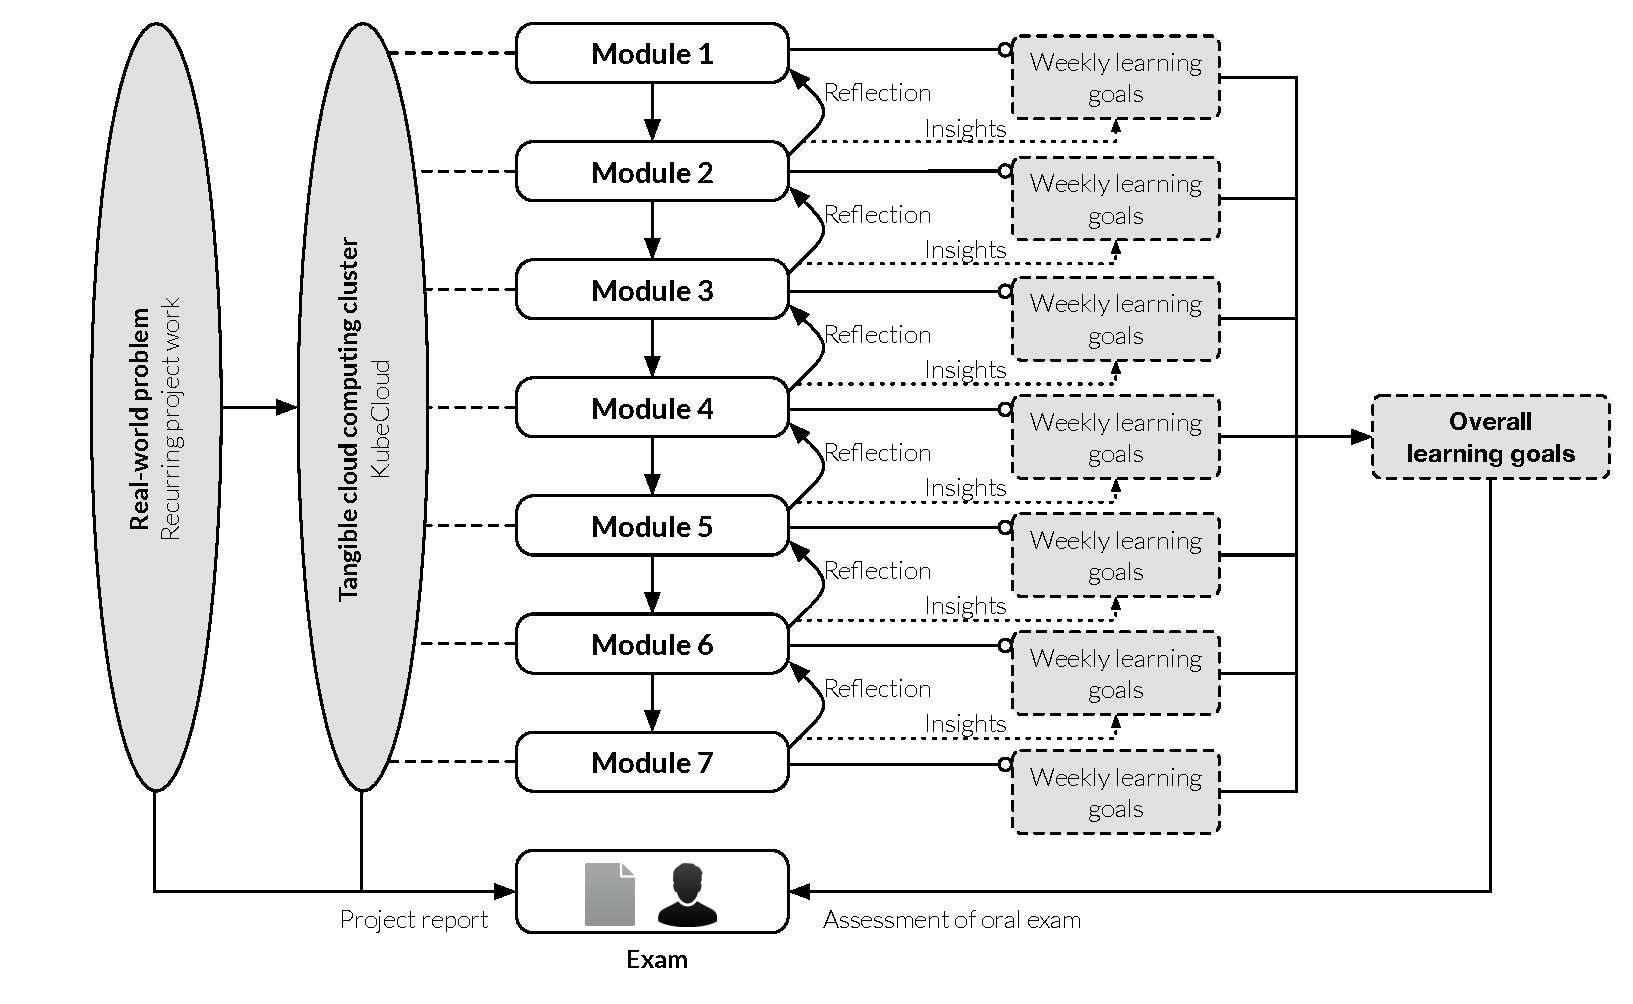
\includegraphics[width=\textwidth]{figures/course_structure}
    \caption{Course Structure}
    \label{fig:course_structure}
\end{figure}


\noindent 
Figure \ref{fig:course_structure} shows the course structure that consists of modules with learning goals connected to an on-going project work phase called "Tangible cloud computing". The project is derived from a real life problem following the principles of PBL. The real-world problem is presented to drive the students' group work. The problem is the e-commerce challenges on Black Friday and is relatively loosely described to allow investigation and experimentation. The problem formulation is shown below.

\begin{kasse} [Problem Formulation]
You are working as a development team within a big e-commerce website company selling goods to all of Scandinavia. Black Friday is getting more and more traction in Scandinavia and for the past two years, you and your team have experienced an increasing traffic on your e-commerce website at midnight when Black Friday begins. Last year 10 minutes past midnight, your application crashed because of the heavy traffic load. You and your team have been assigned a total rewrite of your applications architecture to ensure scalability and resilience. You and your team have chosen to implement the solution as a microservice architecture leveraging the Spring Boot and Spring Cloud frameworks running on the Kubernetes Infrastructure platform where your application is packaged and deployed in containers. The requirements for the solution is fairly simple, but the main focus should be on resilience and scalability. 
\\ \\
\noindent 
The minimum requirements for this problem are as follows:
\begin{itemize}
    \item The application should contain a simple graphical user interface
    \item The application should leverage the gateway API pattern to distribute requests to specific services
    \item The application should contain at least three data delivering services
    \item Services have to be configured remotely so that every client fetches configuration at boot from a central configuration server
\end{itemize}
\end{kasse}


\noindent 
It is seen (Figure \ref{fig:course_structure}) that the learning goals for each module have been created to facilitate the students' learning in order to make it possible to evaluate after each module. The goals are designed with Bloom's taxonomy in mind, with the focus on covering different levels of expertise. \\


\noindent
In order to support the problem-based group work, a tangible cloud computing cluster will be handed out to each group. The cluster acts as a learning object, and it spans several of Churchill's classification of learning objects. Cloud computing is presented as a tangible physical model which both serves as a simulation object and as a conceptual model. Furthermore, it is possible to interact with the cluster and try things out while getting visual feedback. The cluster is supposed to ease the transition from understanding software on a single machine to the scale of a cloud infrastructure. Using the terminology from activity systems, the cluster will work as a mediating tool that, hopefully, is easier to learn and reason about than an actual cloud service provider. Hein describes that the physical actions and hands-on experiences can help learning and that motivation is a key concept. Furthermore, social activity is described as an important factor. \\

\noindent
Questionnaires for each module have been created from the learning goals to evaluate the students' progression and to enforce reflection. The questionnaires contain assessable questions linked to each module's learning goals. The result of the experiment is presented in Chapter~\ref{chapter_experiment1_learning_experience}.

\subsubsection*{Additional Tools and Methods}
Besides the means described above, additional means have been applied to achieve the best possible learning outcome for the students. This section will, in short, present some of the additional methods and tools applied. For further descriptions of these tools, we refer to Appendix~\ref{appendix:a_learning}.

\paragraph{Blog: www.rpi-cloud.com}
A blog has been created with the purpose of sharing the findings during this master's thesis. Furthermore, this blog features articles about different tools such as the Spring Boot and Spring Cloud frameworks used in the course. These articles provide a good basis for the students to get acquainted with the tools used.

\paragraph{Workshops}
Specifically tailored workshops have been created to the topics of Docker (17 pages), Kubernetes (13 pages), and Resilience \& Load testing (19 pages). The workshops supplement the presentations and provide a hands-on approach to the presented topics. Furthermore, these workshops dig deeper into the theory and provide concrete, hands-on experience. 

\paragraph{External Presentation}
In order to relate the concepts taught in the course, an external presenter was invited to bridge the curriculum to the real-world. The external presenter's focus was Continuous Delivery and how tools such as Docker helps in the transitioning to a more service-oriented architecture and the benefits of a continuous delivery pipeline. The presenter, Martin Amdisen, Continuous Delivery Consultant at Praqma, gave the presentation in Module 5.

\paragraph{Additional Activities}
Additional activities cover, among other things, a presentation and demonstration given at the Google Developer Group in Aarhus. Furthermore, a Kubernetes workshop at Praqma in Aarhus was held to introduce some of their employees to Kubernetes. These additional activities support the course's validity and emphasize the demand in the industry for knowledge within these topics.

\subsection*{Assessment}
Assessment refers to determining if the provided means have resulted in the desired learning outcome for the individual student. As mentioned the students are asked to hand in different assignments. On a weekly basis, the students hand in answers to a questionnaire. The questionnaires are designed to give insight into the students' progression along with the possibility of reflecting upon the week's topic seen from the students' perspective. These weekly hand-ins are evaluated using SOLO taxonomy. SOLO taxonomy is chosen because of the nature of the responses given by the students. The answers are fairly short, but they provide insights into the students' progression and understanding of the week's topic and their context in relation to the entire course. SOLO taxonomy provides a useful basis for determining the students' development. The result of these weekly experiments will be presented in Chapter~\ref{chapter_experiment1_learning_experience}.\\

\noindent 
Besides the weekly reflection hand-ins, the students must work with the given project during the entire course. In each week, new tools and theories are added that can be applied in the project work. The students are asked to hand in a report describing the project, how the different topics relate, and how they are implemented in the project. This project will be the foundation for the assessment of the course. The students will present the result individually at an oral exam with a duration of 20 minutes. The students will be assessed by the demonstrated knowledge during these 20 minutes. Bloom's taxonomy will then be used to evaluate the performance, and the outcome of this evaluation will be a grade in the Danish 7-scale system. The date of the exam will be after hand-in of this master's thesis, June 7th, 2016. 

\section{Designing the Weekly Learning Activity}

\noindent
The design of each module will be described in the following using the same structure presented in the previous section. A module consists of 8x45 minutes. Table~\ref{table:material} shows each module's materials, both in terms of reading material, that the students must prepare before class, and the additional resources created within this present master's thesis. Details about the learning material and additional resources can be found in Appendix~\ref{appendix:a_learning}.

\renewcommand*{\arraystretch}{1.8}
\begin{table}[]
\centering

\begin{tabular}{|p{5cm}|p{1cm}|p{1cm}|p{1cm}|p{1cm}|p{1cm}|p{1cm}|p{1cm}|}
\hline
\rowcolor[HTML]{EFEFEF} 
\textbf{Module:}                        & \textbf{1} & \textbf{2} & \textbf{3} & \textbf{4} & \textbf{5} & \multicolumn{1}{l|}{\cellcolor[HTML]{EFEFEF}\textbf{6}} & \textbf{7} \\ \hline
\textbf{Number of slides}               & 123        & 21           & 62           &  58          &   -         &  -                              &  20           \\ \hline
\textbf{Reading materials (pages)}      & 28         & 10           & 44           & 32           & 5           &  -                              &  17          \\ \hline
\textbf{Video (min)}                    & 61         &  10          & 50           & 51           &  0          & -                                & 0           \\ \hline
\textbf{Votiee questions}               & 12         & 0           &  1          & 0           &  0          &   -                             & 0           \\ \hline
\textbf{Workshop (pages)}               & 0          & 17           &  13          & 19           & 0           &  -                              &  0          \\ \hline
\textbf{Number of reflection questions} & 3          & 5           &  7          & 7           & 3           &  -                      & 3           \\ \hline
\end{tabular}
\caption{Overview of Material}
\label{table:material}
\end{table}



\subsection*{Module 1 - Course Introduction and Java Frameworks}

\subsubsection*{Learning Outcome}
The first module will introduce cloud computing, microservice architecture, Raspberry Pi clusters, Spring Boot, and Spring Cloud. The students will get applications up and running locally during the project work. \\

\noindent
On successful completion of this module, students will be able to:
\begin{itemize}
\setlength\itemsep{0.05em}
    \item Understand challenges in cloud computing and microservice architectures by providing sufficient examples
    \item Understand the fundamental anatomy of a cluster by providing sufficient examples
    \item Apply theory of microservice architecture patterns in practice by implementing Java applications using Spring Boot and Spring Cloud 
    \item Evaluate monolithic and microservice architectures by comparing and reflecting upon their benefits and drawback 
\end{itemize}

\subsubsection*{Means}

To achieve the learning outcome of the first module, much material has to be covered. The first four lectures are a combination of presentations combined with small breaks with questions. The students will use a voting platform\footnote{\url{http://www.votiee.com/}} to answer these reflection questions. This approach has been chosen to reach the active learners who need room for reflection and small discussions. Much material is presented in this first module. However, students have 4x45 minutes in the second part of the module to start working with the topics. This distribution of lecturing versus group work is also seen in Table~\ref{table:material} with the number of slides presented.

\subsubsection*{Assessment}
Assessment of the weekly reflection assignment will be evaluated using SOLO taxonomy. The results are described in Chapter~\ref{chapter_experiment1_learning_experience}. 



\subsection*{Module 2 - Docker Lightweight Containers}

\subsubsection*{Learning Outcome}
The second module will cover virtualization by introducing hypervisors and containers, particularly Docker. The project work includes an exercise to create a Docker image of the project from Module 1 to familiarize the students with the technology. \\

\noindent
On successful completion of this module, students will be able to:
\begin{itemize}
        \item Understand virtualization by providing sufficient examples
        \item Understand Docker images and containers by providing sufficient explanations
        \item Apply Docker images and containers by building and running images and containers
        \item Evaluate containers and hypervisors by comparing and reflecting upon their benefits and drawbacks
    \end{itemize}
    
\subsubsection*{Means}
The topic of the second module is, to a larger extent, hands-on with the use of Docker. The presentation is limited to cover only 21 slides as Table~\ref{table:material} shows. Instead, the students are given a workshop to familiarize them with Docker. The workshop supplies the students with a deeper understanding of the use of Docker as a container technology. 

\subsubsection*{Assessment}
Assessment of the weekly reflection assignment will be evaluated using SOLO taxonomy. The results are described in Chapter~\ref{chapter_experiment1_learning_experience}. 

\subsection*{Module 3 - Kubernetes Container Cluster Management}
\subsubsection*{Learning Outcome}
The third module will cover container cluster management by introducing Kubernetes. The project work will include deployment of Docker containers in Kubernetes. \\

\noindent
On successful completion of this module, students will be able to:
\begin{itemize}
    \item Understand the concept of orchestration by providing sufficient explanations
     \item Apply cluster management by deploying Docker containers in a Kubernetes cluster
    \item Analyze Kubernetes' scheduling capabilities by comparing it to manual scheduling
    \item Evaluate Kubernetes' capabilities to sustain uptime by discussing the components of Kubernetes

\end{itemize}

\subsubsection*{Means}
The topic of the third module is cluster management with Kubernetes. Much new material has to be covered because it involves many new concepts. Kubernetes is a central part of the project work, since this is the platform that the students must deploy their microservice architecture in. The presentation of the material is set to approximately two lectures (2x45 min) and includes a live demonstration of a project including visualization of the concepts in KubeCloud. In order to construct the skills needed, the workshop format is used again to familiarize the students with Kubernetes.

\subsubsection*{Assessment}
Assessment of the weekly reflection assignment will be evaluated using SOLO taxonomy. The results are described in Chapter~\ref{chapter_experiment1_learning_experience}. 

\subsection*{Module 4 - Resilience and Load Testing}

\subsubsection*{Learning Outcome}
The fourth module will cover resilience and load testing by introducing and discussing definitions of resilience and load testing. \\

\noindent
On successful completion of this module, students will be able to:
\begin{itemize}
        \item Understand the concept of resilience by providing sufficient examples
        \item Apply patterns to improve resilience by implementing these using Spring Boot and Spring Cloud
        \item Analyze the effect of patterns for resilience by conducting tests agains a cluster using load testing tools
        \item Evaluate testing techniques by comparing stress testing, load testing, and unit testing
    \end{itemize}
    
\subsubsection*{Means}
Resilience and Load testing is covered in a similar manner as in module three. Approximately two lectures (2x45min) consist of presentations and live demonstration of load testing using KubeCloud. Afterwards the students are given a workshop that will highlight the covered topics through experiments.

\subsubsection*{Assessment}
Assessment of the weekly reflection assignment will be evaluated using SOLO taxonomy. The results are described in Chapter~\ref{chapter_experiment1_learning_experience}. 

\subsection*{Module 5 - External Presentation and Project Work}
In the fifth module an external lecturer from industry is invited to present the topic of Continuous Delivery and how its being applied at their customers. The external lecturer is Martin Amdisen, Continuous Delivery Consultant at Praqma. Praqma is a consultancy focusing on helping the industry adopt the principles of Continuous Delivery. The abstract of the talk can be seen below: \\

\noindent\textit{Continuous Delivery is the art of actually getting software to the end users.} \\

\noindent\textit{Praqma is helping many companies large and small get better at releasing their software. With Continuous Delivery we strive to make sure that all code changes end up in the product, thoroughly tested and documented. The key part of this is automation.} \\ 

\noindent\textit{In this talk we will give an introduction to the underlying concepts of Continuous Delivery, as well as a brief overview of some of the tools we use to enable this, such as Docker and Jenkins.} \\

\noindent The remaining time in this module will be used for further development of the project.


\subsection*{Module 6 - Domain Name Service}
The sixth module will introduce DNS. As mentioned earlier this topic will be presented by Pedersen. The content of this talk and the learning goals are specified by Pedersen. The content of this topic is however of utmost importance and is included in the design of the course as part of this master's thesis. The weekly reflection of this module will not be presented in this master's thesis.

\subsection*{Module 7 - Service Discovery and Project Presentation}
\subsubsection*{Learning Outcome}
The seventh module will introduce service discovery, and in the end of the module each group will present their project for the rest of the class. The project work will focus on how to leverage service discovery in Kubernetes on the tangible cloud computing cluster. The topics of Bonjour and Avahi will be covered by another master's thesis student researching these topics.\\ 

\noindent
On successful completion of this module, students will be able to:
\begin{itemize}
    \item Understand service discovery by providing sufficient examples
    \item Analyze service discovery models by comparing when different models are appropriate
    \item Evaluate Bonjour, Avahi and KubeDNS by comparing the similarities and differences between them
\end{itemize}

\subsubsection*{Means}
The topic of this last week of the course cover the topic of Service Discovery and focuses on why it is important and how it is achieved within Kubernetes.

\subsubsection*{Assessment}
Assessment of the weekly reflection assignment will be evaluated using SOLO taxonomy. The results are described in Chapter~\ref{chapter_experiment1_learning_experience}. 

